\documentclass[11pt,a4paper]{article}
\usepackage[T1]{fontenc}
\usepackage[utf8]{inputenc}
\usepackage{lmodern,amsmath,amssymb,amsthm,mathtools,bm}
\usepackage[margin=24mm,headheight=15pt]{geometry}
\usepackage{graphicx,booktabs,array,microtype,xcolor,fancyhdr}
\usepackage[numbers,sort&compress]{natbib}
\usepackage{hyperref}
\hypersetup{colorlinks=true,linkcolor=blue!45!black,citecolor=blue!45!black,urlcolor=blue!45!black,
pdftitle={Hopf-Charge Bounds for Nodal States in Conditional Berger-Hopf Light Transfer},pdfauthor={Norman P. Carberry}}
\pagestyle{fancy}\fancyhf{}
\fancyhead[L]{\small Hopf-charge bounds and light transfer}
\fancyhead[R]{\small Author review draft}\fancyfoot[C]{\thepage}
\setlength{\parskip}{.3em}\setlength{\parindent}{1em}
\setlength{\emergencystretch}{3em}
\renewcommand{\topfraction}{.92}\renewcommand{\textfraction}{.06}
\newtheorem{theorem}{Theorem}\newtheorem{corollary}{Corollary}
\newcommand{\tr}{\operatorname{tr}}\newcommand{\asympart}{\operatorname{Asym}}
\newcommand{\NN}{\mathcal N}\newcommand{\RR}{\mathcal R}
\title{\textbf{Hopf-Charge Bounds for Nodal States in Conditional Berger--Hopf Light Transfer}}
\author{Norman P. Carberry\\\small Independent Researcher, Oconomowoc, Wisconsin, USA\\
\small ORCID: \href{https://orcid.org/0009-0000-6650-3485}{0009-0000-6650-3485}}
\date{}
\begin{document}
\maketitle
\begin{center}\small Research article draft for \emph{Galaxies}: Strong Gravitational Lens Modeling\end{center}
\begin{abstract}
A scalar preparation can leave a fiducial light ray undeflected at first
order while deforming its neighboring beam. We determine the Hopf content
required by this nodal construction in the degree-two scalar sector of
the three-sphere. For a nonzero normalized quadratic harmonic whose value
and full spatial gradient vanish on a great circle, the squared-norm
fraction in absolute Hopf charge two is exactly $(1+\kappa^2)/2\ge1/2$,
where $\kappa$ is the absolute K\"ahler cosine of the ray plane. A Hopf-fibre
ray requires a purely charged state. The result fixes its Berger Dirichlet
Rayleigh quotient and gives a rigidity criterion for persistence of the
node under an explicitly specified scalar spectral action. We apply the
normalized nodal family to a separately declared round-background
scalar--tensor realization used in the Berger--Hopf program. Its full
six-coordinate state determines incoming, outgoing and observer--source
Jacobi responses, fixed-physical-source timing shifts, and an evaluated
antisymmetric ordered-transfer kernel for independent angular histories.
The kernel is absent in a common-profile preparation. General lensing
theory nevertheless permits a common affine source transformation that
symmetrizes the strong-lens maps in the tidal approximation. The advance
is a sharp geometric restriction on the preparation and a reproducible
conditional response family; it supplies neither a microscopic
action-to-cosmology identification nor a unique observable amplitude.
\end{abstract}
\noindent\textbf{Keywords:} strong gravitational lensing; Hopf fibration;
Berger sphere; scalar harmonics; Jacobi map; time delay

\section{Physical question and scope}

The Berger--Hopf Standard Model (BHSM) research program organizes physical
responses around envelope geometry, boundary matching and a constrained
action. In a lensing application, an effective gravitational potential may
represent the same contribution as an envelope description. A useful result
therefore need not depart from general relativity, but it must determine
something beyond assigning an arbitrary angular profile and amplitude.

The starting angular calculation used normalized degree-two harmonics of a
round closed background and a specified six-coordinate scalar--fluid state
\cite{Carberry2026EnvironmentalSource,Carberry2026TransportSource}.
One preparation has a central spatial ray on which the scalar value and
its first derivatives vanish, while a nonzero transverse Hessian changes
the beam. The resulting fixed-source singular-isothermal-sphere (SIS)
delay is linked to incoming and total-path shear. That is a conditional
effective-model calculation. A quadrupolar $\cos2\varphi$ pattern, by itself,
does not establish a Hopf-fibre effect or a physical state selection.

We ask a more restrictive question: \emph{what Hopf representation content
must that nodal preparation have?} Theorem~\ref{thm:charge} answers it
without choosing a numerical amplitude. Its sharp half-power bound holds
for every orthogonal Hopf structure; the precise fraction depends on the
relative orientation of the ray plane. A second theorem states exactly
when the same node can persist for a free scalar on a fixed Berger space.
These are spatial geometry and explicitly specified scalar-action results.
The cosmological optical application remains on the separate round branch.

The scalar Berger spectrum is known \cite{Lauret2019Berger}. The harmonic
and full-sky shear machinery is established
\cite{Lindblom2017Harmonics,Bernardeau2010FullSky}. Distance-matrix lens
equations, arrival times and equivalent-lens freedom are also established
\cite{Schneider1997Equivalent,Fleury2021Arbitrary,Schneider2019Multiplane}.
Our addition is the sharp constrained charge fraction, its nodal-persistence
consequence, and the evaluated state response for the declared optical
realization. The general ordered-tide rotation mechanism is already derived
in the literature, including a closely related recent Jacobi-map treatment
\cite{Magi2026Rotation}; we use it as a checkable response channel.

No unique microscopic BHSM reduction to the chosen scalar--tensor action
is assumed. The recovered boundary/Hessian machinery identifies concrete
common-domain projection requirements, but does not evaluate that bridge.
The microscopic fixed-external-label condition also does not impose
alignment of cosmological angular states. These distinctions motivate the
state family used here. The source archive contains the finite recovery map,
hashes and reconciliation, rather than treating an unlocated object as a
proof that it was never derived.

\section{Normalized spatial state and Hopf structure}
\label{sec:geometry}

Let $S^3$ be the unit sphere embedded in $\mathbb R^4$, with coordinates
$X$. Write the physical round spatial metric as $R^2h_1$, $K=R^{-2}$,
and consider a real symmetric tracefree matrix $A$. Define
\begin{equation}
 F_A(X)=X^TAX,\qquad Q_A=\NN F_A,
 \qquad \NN=\sqrt{6/(\pi^2R^3)}.
 \label{eq:normalization}
\end{equation}
Restriction of a homogeneous harmonic quadratic gives
$-\Delta_{R^2h_1}Q_A=8KQ_A$. The fourth moment of normalized round
measure is
\begin{equation}
 \int X_iX_jX_kX_l\,d\mu=
 (\delta_{ij}\delta_{kl}+\delta_{ik}\delta_{jl}
 +\delta_{il}\delta_{jk})/24.
\end{equation}
Consequently $\int F_AF_Bd\mu=\tr(AB)/12$ and
$\int Q_AQ_BdV_{R^2h_1}=\tr(AB)$. Frobenius-orthonormal STF matrices
thus give nine orthonormal scalar harmonics. Observer-centered sky
decomposition gives one monopole, three dipoles and five quadrupoles;
the degree $n=2$ on $S^3$ must be distinguished from sky angular degree.

An orthogonal complex structure $J$ satisfies $J^T=-J$, $J^2=-I$.
Its Hopf flow is $X\mapsto e^{\theta J}X$, generated by $\xi=JX$.
The orthogonal involution $A\mapsto J^TAJ$ gives
\begin{equation}
 A_0=\tfrac12(A+J^TAJ),\qquad
 A_2=\tfrac12(A-J^TAJ).
 \label{eq:projectors}
\end{equation}
The neutral subspace has real dimension three; it obeys $[A_0,J]=0$
and $\xi F_{A_0}=0$. The charged subspace has dimension six, obeys
$\{A_2,J\}=0$ and $\xi^2F_{A_2}=-4F_{A_2}$. The latter real
space contains the charges $q=\pm2$ together. The power fraction
\begin{equation}
 f_2(A;J)=\|A_2\|_F^2/\|A\|_F^2
 \label{eq:f2}
\end{equation}
is therefore a normalized scalar $L^2$ fraction, not an observed mass
fraction or a probability distribution over envelopes. At the round
point a preferred $J$ is not dynamically selected by isotropy.

\section{The stationary-nodal charge bound}

Let $P$ be a real two-plane and $W=P^\perp$. Its great circle is
$P\cap S^3$. We require both $F_A=0$ and the \emph{full} spherical
gradient $\nabla F_A=0$ on that circle. Requiring only a derivative
tangent to the circle would impose no such restriction.

\begin{theorem}[Sharp charge fraction]
\label{thm:charge}
For nonzero symmetric tracefree $A$ stationary-nodal on $P\cap S^3$,
let $e_1,e_2$ be an orthonormal basis of $W$ and set
$\kappa=|e_1^TJe_2|$. Then
\begin{equation}
 \boxed{f_2(A;J)=\frac{1+\kappa^2}{2}\in[1/2,1].}
 \label{eq:bound}
\end{equation}
The absolute K\"ahler cosine of $P$ equals that of $W$ in real dimension four.
The result is independent of the transverse amplitude and orientation
of $A$. The upper endpoint holds exactly when $P$ is $J$-invariant,
so that its nodal circle is a Hopf fibre. The lower endpoint is attained
by a totally real plane.
\end{theorem}

\begin{proof}
On the unit sphere, $\nabla F_A=2(AX-F_AX)$. Simultaneous vanishing
of value and gradient gives $AX=0$. An open arc spans $P$, so $A|_P=0$.
Symmetry and trace freedom then give, in the splitting $W\oplus P$,
\begin{equation}
 A=C\oplus0,\qquad
 C=\begin{pmatrix}p&q\\q&-p\end{pmatrix}\ne0.
 \label{eq:screenC}
\end{equation}
The compression of the skew matrix $J$ to $W$ is
$J_{WW}=j\left(\begin{smallmatrix}0&1\\-1&0\end{smallmatrix}\right)$,
where $|j|=\kappa$. Direct multiplication gives
\begin{equation}
 \tr(AJ^TAJ)=\tr(CJ_{WW}^TCJ_{WW})
 =-\kappa^2\tr(C^2).
 \label{eq:traceidentity}
\end{equation}
Since the involution preserves the Frobenius norm,
$\|A_2\|^2=(\|A\|^2-\langle A,J^TAJ\rangle)/2$, proving
Eq.~\eqref{eq:bound}. Orthogonality of $J$ gives $\kappa\le1$.
Equality implies $J(W)=W$, equivalently $J(P)=P$. Conversely such
invariance gives $\kappa=1$. Totally real $P$ has $\kappa=0$.
Both endpoints admit nonzero matrices~\eqref{eq:screenC}.
\end{proof}

The theorem is stronger than a chosen ``Hopf-neutral'' restriction:
no Hopf orientation makes this nonzero nodal family neutral. Every
instantaneous nonzero combination of the two transverse tensors in
Eq.~\eqref{eq:screenC} has the same fraction for fixed $P,J$. Independent
temporal histories therefore do not invalidate the spatial bound.
This applies to the fixed nodal subspace; finely adjusted cancellations
along a spacetime trajectory with unrelated time-varying spatial tensors
are not covered by the hypothesis.

\subsection{Exact spectral consequence and scale convention}

Use the Berger family
\begin{equation}
 h_{a,R}=R^2(h_H+a^{-2}\eta^2),\qquad
 -\Delta_{a,R}=R^{-2}[-\Delta_1-(a^2-1)\xi^2],\quad a>0.
 \label{eq:berger}
\end{equation}
Here $a$ is the inverse relative fibre scale and $R$ the horizontal
radius, distinct from the cosmological scale factor below. The known
scalar spectrum is $R^{-2}[k(k+2)+(a^2-1)q^2]$
\cite{Lauret2019Berger}. Thus $n=2$ splits into $8/R^2$ and
$(4+4a^2)/R^2$. The volume differs from round volume by the constant
$a^{-1}$, so normalized measure and power fractions are unchanged.

For fixed $A,R$ the exact Dirichlet Rayleigh quotient is
\begin{equation}
 \boxed{\RR_a[A]=\frac{8+4(a^2-1)f_2}{R^2},\qquad
 \frac{\partial\RR_a}{\partial(a^2)}\bigg|_{A,R}
 =\frac{2(1+\kappa^2)}{R^2}.}
 \label{eq:rayleigh}
\end{equation}
This derivative lies between $2/R^2$ and $4/R^2$. A mixed-sector
function is generally not an eigenfunction when $a\ne1$; the quotient
must not be relabeled an eigenvalue. For $a>1$, the quotient lies
between $(6+2a^2)/R^2$ and $(4+4a^2)/R^2$; their ordering reverses
for $a<1$. All reunite at $8/R^2$ when $a=1$.

The held scale matters. Fixed volume instead requires
$R(a)=R_0a^{1/3}$; at $a=1$ the derivative with respect to $a^2$
becomes $(4f_2-8/3)/R_0^2$, which can be negative. Equation~\eqref{eq:rayleigh}
is a fixed-horizontal-radius statement, not a scale-independent lower
bound on the full BHSM envelope energy. Other terms in a physical
action may modify its energy and dynamics.

\begin{figure}[tbp]\centering
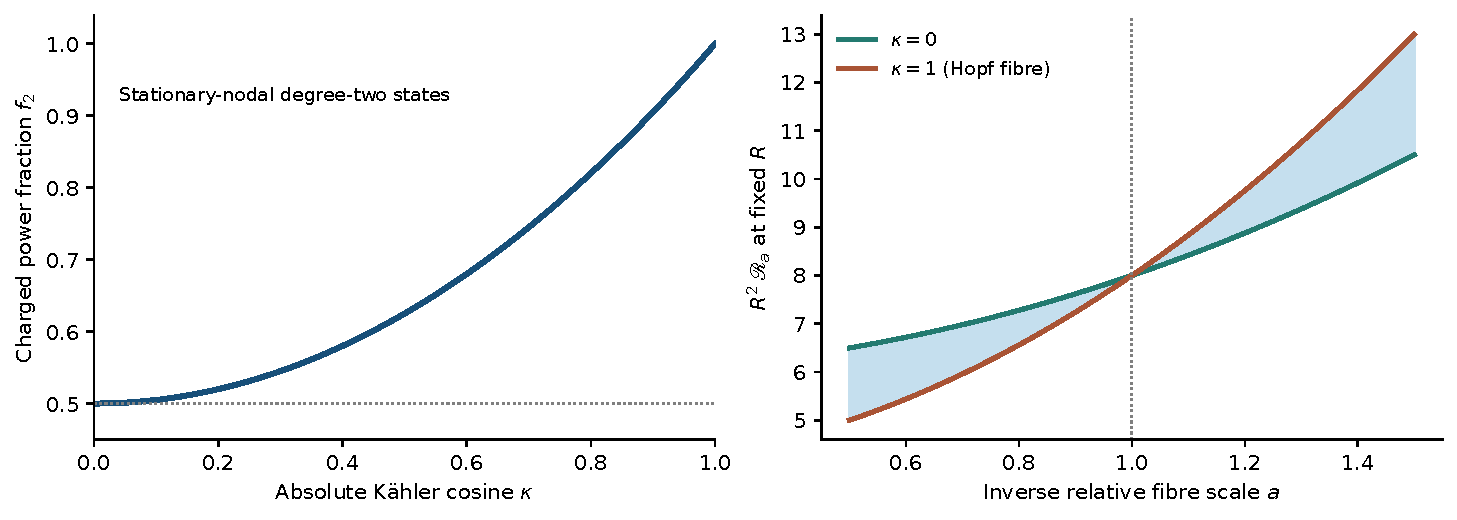
\includegraphics[width=.98\linewidth]{../figures/hopf_bound.pdf}
\caption{Exact geometric restriction, with no fitted physical amplitude.
Left: mandatory charged fraction against $\kappa$. Right: fixed-horizontal-
radius Dirichlet Rayleigh quotient for the stationary-nodal family.
The shaded region spans all Hopf orientations and is not a confidence band.
Neither panel computes squashed-spacetime light propagation.}
\label{fig:hopf}
\end{figure}

\subsection{A specified action and persistence of the node}

An auxiliary test action makes the dynamical limitation explicit:
\begin{equation}
 S_{\rm test}=\tfrac12\int dt\left[
 \|\dot F\|_{L^2(d\mu)}^2-\langle F,-\Delta_{a,R}F\rangle_{d\mu}\right].
 \label{eq:testaction}
\end{equation}
It describes a free scalar on a fixed product time--Berger space, in
units with wave speed one. Variation gives $\ddot F-\Delta_{a,R}F=0$.
The degree-two subspace is invariant under this exact operator, so its
finite reduction is justified without an arbitrary projected stiffness.
This action is an explicit auxiliary realization, not the cosmological
R1 action or a derived microscopic envelope action.

\begin{theorem}[Nodal persistence]
\label{thm:persistence}
For $a\ne1$, a nonzero degree-two solution of
Eq.~\eqref{eq:testaction} can remain stationary-nodal on one fixed
great circle throughout a time interval only if that circle is a Hopf
fibre. If it is a Hopf fibre, its nodal subspace is invariant.
\end{theorem}
\begin{proof}
Write $\mathcal V(P)=\{A=A^T,\tr A=0,A|_P=0\}$. If $A(t)$ stays
in this linear space then $\ddot A(t)$ does too. The equation and
$a^2-1\ne0$ imply $A_2(t)\in\mathcal V(P)$, hence
$A_0(t)\in\mathcal V(P)$. Theorem~\ref{thm:charge} excludes any
nonzero neutral element of $\mathcal V(P)$. Thus every nonzero
$A(t)$ is entirely charged, and Eq.~\eqref{eq:bound} forces
$\kappa=1$. Conversely $\kappa=1$ makes every element entirely
charged, on which the Laplacian is a scalar, preserving the subspace.
\end{proof}

The round case is an essential exception. For $a=1$ both sectors
evolve with the same operator, and every nodal plane is allowed.
The zero solution and isolated nodal instants do not contradict the
theorem. Operators that mix sectors, change $J$ or the ray plane, or
have additional field constraints require their own analysis. Thus
persisting with the old nodal ansatz after squashing is a physical
restriction, not an automatic continuation of round cosmology.

\section{Conditional round-background action-to-light map}
\label{sec:optics}

We next use the previously specified R1 action as a concrete optical
realization on the round closed background. In code units
$M_{\rm Pl}=H_0=c=1$,
\begin{equation}
 S_{\rm R1}=\int d^4x\sqrt{-g}\left[
 \frac{\mathcal R}{2}+X-V_0+q_TT-\frac{2X}{\lambda}\Box T\right]+S_m+S_r,
 \qquad X=-\tfrac12(\nabla T)^2.
 \label{eq:r1}
\end{equation}
This is an established kinetic-gravity-braiding action class
\cite{Deffayet2010Braiding,Kobayashi2011Generalized}, with minimally
coupled irrotational dust and radiation. Its parameters are fixed:
$(\Omega_{m0},\Omega_{r0},\Omega_{k0},\lambda,q_T)
=(0.31,9\times10^{-5},-0.018,1,3)$ and
$V_0=2.3986073449708067$. They are not fitted to lens data.
Appendix~\ref{app:action-provider} supplies the background, full finite
action, constraints, normalization and canonical equations.

In uniform-field gauge, the auxiliary lapse, shift and fluid velocities
are algebraically solved using their actual action block $A_{\rm aux}$.
The reduced kinetic block is $M=M_0-B^TA_{\rm aux}^{-1}B$.
The physical degree-two mode has no homogeneous or pure-gauge dipole
direction left to invert. The six-dimensional canonical state is
$(x,p)$ with $x=(\zeta,D_m,D_r)$ and
$p=a_{\rm cos}^3(M\dot x+Lx)$, where $a_{\rm cos}=e^N$.
No pseudoinverse of a gauge zero mode is used. Nonflat scalar constraints
must be retained; replacing this reduction by a flat sound-speed equation
would not follow from the closed Horndeski action \cite{Akama2019Nonflat}.

At $z_i=2.1$ the specified physical coordinates are
\begin{equation}
 y=(\zeta,\Pi_{2,\rm ref},\delta_m^{\rm ADM},\delta_r^{\rm ADM},
 v_m^{\rm ADM},v_r^{\rm ADM})_i^T.
 \label{eq:anchor}
\end{equation}
The reference $\Pi$ is not the full coupled canonical momentum.
An invertible six-row map $\mathcal B_i$ converts the physical anchor
to the canonical state. The action fixes $U'=F(N)U$, $U(N_i)=I$,
and the Newtonian reconstruction rows fix
\begin{equation}
 w(N)=(\phi+\psi)(N)\,U(N,N_i)\mathcal B_i^{-1},\quad
 ds^2=a_{\rm cos}^2[-(1+2\Phi)d\eta^2+(1-2\Psi)\gamma_{ij}dx^idx^j].
 \label{eq:weyl}
\end{equation}
Thus $w\cdot y$ is the Weyl-potential coefficient of one normalized
harmonic. The same temporal transfer applies to each of nine independent
spatial harmonics on the round branch. This gives 54 initial coordinates,
not an automatically aligned single profile. No action principle here
selects these initial data.

\subsection{Nodal tensors and three propagation segments}

For a fiducial observer--radial ray take
$P=\operatorname{span}(e_0,e_3)$ and parallel transverse screen
$(e_1,e_2)$. Let $Z=\operatorname{diag}(1,-1)$,
$X=\left(\begin{smallmatrix}0&1\\1&0\end{smallmatrix}\right)$ and
choose unit tensors $A_+=(Z/\sqrt2)\oplus0$ and
$A_\times=(X/\sqrt2)\oplus0$ on $W\oplus P$. Their screen Hessians are
\begin{equation}
 (D_\perp D_\perp Q_+)_{\rm TF}=\sqrt2\NN KZ,\qquad
 (D_\perp D_\perp Q_\times)_{\rm TF}=\sqrt2\NN KX.
 \label{eq:hessians}
\end{equation}
Both have zero value, full first derivative and screen Hessian trace
along the central ray. First-order radial/frequency, endpoint and local
frame terms therefore vanish for this preparation, while the beam
deforms. These properties are spatial statements on the round branch.

For independent six-coordinate inputs $u,v$ in these two tensors, define
$S_K(r)=\sin(\sqrt K r)/\sqrt K$. For vertices $a<b$, the background
physical angular-diameter distance is
$d_{ab}=a_{{\rm cos},b}S_K(\chi_b-\chi_a)$. The action-derived shear is
\begin{align}
 D_{ab}&=d_{ab}(I-\Gamma_{ab})+O(y^2),\nonumber\\
 \Gamma_{ab}&=\sqrt2[(g_{ab}\cdot u)Z+(g_{ab}\cdot v)X],
 \label{eq:gamma}\\
 g_{ab}&=\frac{\NN K}{S_K(\chi_b-\chi_a)}
 \int_{\chi_a}^{\chi_b}S_K(\chi_b-t)S_K(t-\chi_a)w(t)\,dt .
 \label{eq:g}
\end{align}
Lengths use $c/H_0$; the volume-normalized $Q$ and field coefficients
use those same units. No extra observer--vertex scale factor is added.
All three maps $ol$, $os$, $ls$ use the same state, but each has its
own vertex conditions. In particular $D_{ls}\ne D_{os}-D_{ol}$.

This completes the conditional optical chain: the supplied effective
action fixes a constrained, normalized propagator; its metric rows and
the exact spatial Hessian fix incoming/local/outgoing transfer. The
geometric theorem restricts the allowed nodal shapes. The missing
microscopic identification is an earlier arrow, which this calculation
does not replace with a free coefficient or a second copy of gravity.

\section{Independent histories and ordered transfer}
\label{sec:rotation}

With $c_*=\sqrt2\NN K$, the conformal screen equation is
\begin{equation}
 D''+KD=-\epsilon\mathcal T_1D+O(\epsilon^2),\qquad
 \mathcal T_1=c_*[(w\cdot u)Z+(w\cdot v)X],\quad
 D(a)=0,\ D'(a)=I.
 \label{eq:jacobi}
\end{equation}
Here $\epsilon$ scales both inputs. In a consistently parallel
orthonormal screen, every optical tidal coefficient is symmetric.
Expanding $D=S_K I+\epsilon D_1+\epsilon^2D_2+\cdots$, an arbitrary
second-order tidal term multiplies $S_K I$ and contributes only a
symmetric part to $D_2$. The ordered product of first-order tides gives
\begin{align}
 \asympart\frac{D_{ab}}{S_K(b-a)}
 &=\epsilon^2(u^T\mathsf B_{ab}v)J_s+O(\epsilon^3),\quad J_s=ZX,
 \label{eq:bilinear}\\
 (\mathsf B_{ab})_{ij}
 &=\frac{c_*^2}{S_K(b-a)}\int_a^bdt\int_a^tds\,
 S_K(b-t)S_K(t-s)S_K(s-a)\nonumber\\[-2pt]
 &\hspace{25mm}\times[w_i(t)w_j(s)-w_j(t)w_i(s)].
 \label{eq:B}
\end{align}
Thus $\mathsf B^T=-\mathsf B$. If $v=ru$, all tides commute and
the rotation vanishes exactly in the finite first-order-tide ODE.
The converse need not hold: independent histories can cancel in a
particular integral. Numerical singular values are basis-dependent
and do not define a physical energy norm.

Equation~\eqref{eq:B} is the known ordered-tide mechanism, now evaluated
on the normalized R1 state \cite{Magi2026Rotation}. It describes map
antisymmetry, not optical twist: $D^TD'-D'^TD=0$, so $D'D^{-1}$ is
symmetric where defined. Fixed-redshift endpoint shifts add symmetric
terms at this order. A separately rotated source screen changes the
matrix representation and must not be counted as a new signal.
The independence from unknown second-order tidal terms applies to an
isotropic \emph{smooth} baseline. It does not give the complete
second-order response after an order-one anisotropic local lens.

For numerical evaluation, the first-order positive-response row $G$
and unnormalized $B$ obey
\begin{equation}
 G''+KG=c_*wS_K(t-a),\qquad
 B''+KB=c_*(wG^T-Gw^T),
 \label{eq:responseode}
\end{equation}
with zero initial data, and $\mathsf B=B(b)/S_K(b-a)$.
Independent ordered quadrature and direct matrix-ODE integration test
this reduction. An even-amplitude projection isolates the quadratic
coefficient. For the finite tracefree-tide ODE only even orders have
antisymmetric parts. A Volterra majorant bounds higher even terms by
\begin{equation}
 \frac{L}{S_K(L)}\sum_{m\ge2}\frac{\nu^{2m}}{(4m+1)!},\qquad
 \nu=L^2\sup\|\mathcal T_1\|,\quad L=b-a,
 \label{eq:majorant}
\end{equation}
using $0\le S_K(r)\le r$ before the first conjugate point. It controls
the declared optical equation; it is not a bound on omitted nonlinear
field equations. The supplied numerical maximum is sampled rather
than interval-certified.

\section{Strong-lensing timing and representation freedom}
\label{sec:lens}

For a fixed physical local potential $\widehat\psi$, source displacement
$X_s$ and measured redshifts, standard distance-matrix theory gives
\begin{align}
 \beta&=D_{os}^{-1}X_s,\qquad
 \mathsf T=(1+z_l)D_{ol}^TD_{ls}^{-1}D_{os},\nonumber\\
 ct(\theta)&=\tfrac12(\theta-\beta)^T\mathsf T(\theta-\beta)
 -(1+z_l)\widehat\psi(D_{ol}\theta)+f(\beta).
 \label{eq:fermat}
\end{align}
The matrix $\mathsf T$ is symmetric by optical reciprocity
\cite{Fleury2021Arbitrary}. For $D_{ab}=d_{ab}(I+E_{ab})$,
$\delta\mathsf T/\mathsf T_0=E_{ol}+E_{os}-E_{ls}$.
Stationarity of an image removes its positional variation from the
first derivative of arrival time. With $q_i=\theta_i-\beta$,
\begin{equation}
 \frac{c\,\delta t_i-\delta f}{T_0}
 =\tfrac12q_i^T(E_{os}-E_{ol}-E_{ls})q_i
 +q_i^T(E_{os}-E_{ol})\beta .
 \label{eq:dt}
\end{equation}
This includes the changing source angle and impact in the fixed physical
lens. Holding angular source position fixed would give a different law.

For an SIS $\widehat\psi(x)=b|x|$, physical source offset $s e$,
$e=(\cos\varphi,\sin\varphi)$, and noncritical two-image branches,
the quadratic term cancels between images. Therefore
\begin{align}
 \Delta t_0&=\frac{2(1+z_l)bs}{c}\frac{d_{ol}}{d_{os}},\nonumber\\
 \frac{\delta\Delta t}{\Delta t_0}
 &=\sqrt2[(g_{os}-g_{ol})\cdot u\cos2\varphi
 +(g_{os}-g_{ol})\cdot v\sin2\varphi].
 \label{eq:sis}
\end{align}
The $ls$ shear cancels from this particular timing derivative, while
remaining in image positions. The earlier common $+$ seed is recovered
by setting $v=0$. The angular pattern is inherited scalar shear geometry;
the geometric result here concerns its mandatory Hopf content.

There is also a leading rotation in a chosen angular source chart.
For a prescribed fixed symmetric reduced local-lens Hessian $L$, put
$F=\Gamma_{ol}+\Gamma_{os}-\Gamma_{ls}$. The angular-source Jacobian
$A_{\rm ang}=I-D_{os}^{-1}D_{ls}\widehat\psi''D_{ol}$ has
\begin{equation}
 \delta A_{\rm ang}=-(\Gamma_{os}-\Gamma_{ls})L+L\Gamma_{ol}.
 \label{eq:lensrotation}
\end{equation}
Resampling a general lens at a shifted impact also adds a symmetric
$-\delta L$, leaving the displayed antisymmetric part unchanged.
The Jacobian can be nonsymmetric at first order because the main lens is already
anisotropic at order zero. This is distinct from the quadratic smooth
rotation in Eq.~\eqref{eq:bilinear}.

Neither raw antisymmetry supplies a source-independent identification.
For common transfer matrices across all images, the physical-source
Jacobian at image $i$ is $A_i=D_{os}-D_{ls}U_iD_{ol}$, with symmetric
$U_i$. One common affine source transformation gives
\begin{equation}
 \underbrace{D_{ol}^TD_{ls}^{-1}}_{\mathcal S}A_i
 =D_{ol}^TD_{ls}^{-1}D_{os}-D_{ol}^TU_iD_{ol},
 \label{eq:symmetrizer}
\end{equation}
which is symmetric for every image. This is the equivalent-lens freedom
\cite{Schneider1997Equivalent,Fleury2021Arbitrary}, and is consistent
with $\mathsf T A_{\rm ang}$ being a Fermat Hessian. The effective
potential represents the same surface contribution; adding another copy
would double count it. Restricted source/lens calibration or genuinely
ray-dependent transfers are required to identify additional physics.
Mass-sheet and source-position freedoms remain
\cite{Schneider2019Multiplane,SchneiderSluse2014SPT}; multiple source
redshifts alone do not remove them.

\section{Executed checks and limits}
\label{sec:checks}

The geometric proof is exact. The package independently verifies the
projector dimensions, trace identity, full-gradient nodal condition and
Berger operator action symbolically, and tests both orientation classes
of $J$ numerically. It includes endpoint examples and spectral values on
both sides of the round point. The auxiliary-action check compares its
exact two-sector evolution with the claimed nodal persistence criterion.

The recovered nine-stage angular calculation was replayed from its
original provider hashes. Its chosen matter coefficient
$u=(0,0,10^{-3},0,0,0)$, $v=0$, $\sigma_v=200$ km/s and fixed
$s=0.8$ kpc give $\Delta t_0=7.753621449$ days and
$\delta\Delta t=-0.353216090\cos2\varphi$ s at $(z_l,z_s)=(0.3,1)$.
These are forward-model values, not measured amplitudes.

For independent nodal histories the new kernel retains all fifteen
distinct coordinate-pair coefficients in its machine-readable output.
Two illustrations use $u=10^{-3}e_2$ and either $v=10^{-3}e_3$
(matter/radiation density) or $v=10^{-3}e_1$ (reference scalar momentum),
with zero-based coordinate indices from Eq.~\eqref{eq:anchor}.
At $z_s=1$ the smooth normalized rotation coefficients are, respectively,
\begin{equation}
 \omega^{(2)}_{mr}=-9.98254\times10^{-19},\qquad
 \omega^{(2)}_{m\Pi}=6.70644\times10^{-14}.
 \label{eq:values}
\end{equation}
The tiny density-pair result is retained. The larger response is a
different coordinate probe with a different physical preparation; no
amplitude is selected to match an observation.

\begin{figure}[tbp]\centering
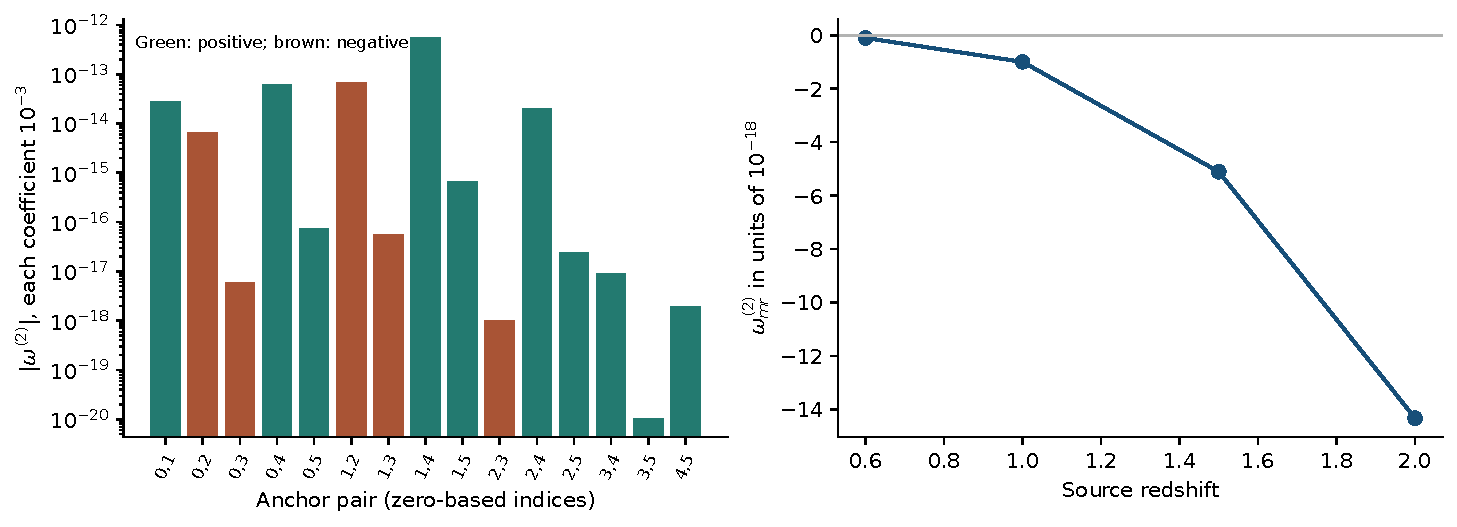
\includegraphics[width=.98\linewidth]{../figures/state_response.pdf}
\caption{Conditional state responses on the round R1 branch. Left: all
fifteen absolute pair responses at $z_s=1$ for $10^{-3}$ in each indicated
anchor coordinate; signs and the full matrix are in the supplied JSON.
Coordinate magnitudes are not comparable physical energies. Right:
smooth ordered rotation for the stated density pair across source
redshifts; the marker at $z_s=1$ matches Eq.~\eqref{eq:values}.
These are parallel-screen transfer coefficients, not detection forecasts.}
\label{fig:states}
\end{figure}

For the density pair, 801-point ordered quadrature and the response ODE
agree in $u^T\mathsf Bv$ to $5.2\times10^{-29}$; refining the temporal
provider from 801 to 1601 samples and tightening the propagator changes
it by $1.3\times10^{-28}$. Direct finite matrix-ODE checks agree with
the coefficient within $4.3\times10^{-26}$ over the stated amplitude
scales. The common-profile finite check is consistent with zero at
$3.4\times10^{-21}$ absolute map antisymmetry. Independent synthetic
time-varying tides check the sign, amplitude convergence and zero-twist
Wronskian without using the R1 response implementation.

For the illustrative density pair, sampled $\nu=6.56\times10^{-6}$
gives a higher-even-order majorant about $5.11\times10^{-27}$ in the
specified first-order-tide ODE. Floating-point cancellation dominates
the smallest direct differences; the larger reported differences are
kept as numerical limitations. Arbitrary symmetric second-order test
tides leave the limiting quadratic rotation unchanged, as the derivation
requires. They are diagnostic forcings, not physical second-order fields.

On 161 time samples from $z_i=2.1$ to zero, the reduced kinetic block
has minimum eigenvalue $2.485\times10^{-3}$ and the auxiliary block has
maximum condition number $1.03\times10^5$. Original constraint residuals
are at most $2.92\times10^{-11}$ in the recorded scaled test, and the
physical anchor reconstruction error is $2.23\times10^{-16}$. Sampled
global angular bounds on $|\Phi|,|\Psi|$ across that full time interval
are below $4.35\times10^{-4}$ for the density pair and $1.90\times10^{-3}$
for the momentum illustration. These support a weak perturbative example
in the tested domain; they do not certify continuum stability, nonlinear
admission or a unique physical state. A successful solve of an auxiliary
block is not a ghost/stability proof.

As a fixed-lens illustration take reduced local convergence $0.45$,
shear amplitude $0.35$ and axis $0.31$ radians at $(z_l,z_s)=(0.3,1)$.
For the density pair Eq.~\eqref{eq:lensrotation} gives angular-source
antisymmetric coefficient $6.82191\times10^{-8}$; centered finite
differencing agrees to $1.93\times10^{-15}$. Its Fermat-weighted
antisymmetric derivative vanishes to rounding, as required by
Eq.~\eqref{eq:symmetrizer}. This is a representation check with
prescribed local inputs, not an inferred astronomical rotation.

\section{Scientific benefit and remaining physical freedom}

The sharp bound supplies a genuine restriction that was absent from
the supplied angular seed: shear with a structurally stationary nodal
degree-two ray necessarily involves Hopf-charged modes. On a Hopf-fibre
ray it is entirely charged; elsewhere its mixed sectors have a specified
fraction and cannot preserve the same node under the auxiliary split
spectral dynamics. This tells a subsequent nonround action calculation
which state restrictions it must respect, rather than treating the
round node as a generic Berger configuration.

The optical calculation supplies a state family instead of inventing a
vacuum or aligning environmental data to obtain a desired number.
Independent histories open a noncommuting transfer channel, but the
established equivalent-lens freedom limits what that channel can mean
without calibrated sources and lenses. The small coefficients in the
examples give no basis for a detection forecast. No stochastic ensemble,
survey likelihood or fresh observational validation is supplied.

The microscopic-to-R1 identification remains a specific missing object:
an evaluated common-domain normalized action, background, constrained
source pairing and metric/phase projection that identifies the exported
BHSM field with the cosmological state and its admissible boundary data.
The recovered Schur contracts and microscopic interface derivatives do
not by themselves provide it. A complete squashed-spacetime application
would additionally require a consistent nonround background, constraints,
state evolution, parallel-screen ray and metric response. Substituting
Berger eigenvalues into the isotropic R1 equations is not that derivation.

Relative to the known spectrum \cite{Lauret2019Berger}, this work proves
the constrained fraction and its persistence consequence. Relative to
the general lensing and second-order rotation treatments
\cite{Fleury2021Arbitrary,Magi2026Rotation}, it evaluates a normalized
conditional state operator and verifies its source-remapping limit.
These are bounded theoretical/computational additions, not a new general
lensing principle or the completion of BHSM. Their scientific value is
that the assumptions and remaining freedoms are explicit enough to test.

\appendix
\section{Frozen effective action and six-state temporal provider}
\label{app:action-provider}

This appendix specifies the conditional R1 realization used for the temporal
response coefficients.  It retains the coupled scalar, dust, and radiation
system of the environmental and transport source calculations
\cite{Carberry2026EnvironmentalSource,Carberry2026TransportSource}.
It does not infer the microscopic BHSM state or its absolute normalization.
The vendored source files and their hashes identify the precise implementation;
only the background entries of the inherited parameter manifest are used.

\subsection{Action, units, and background}

The metric signature is $(-,+,+,+)$ and dots denote cosmic-time derivatives.
In the code units $H_0=M_{\mathrm{Pl}}=c=1$, the effective action, up to its
constant dimensional prefactor, is
\begin{equation}
 S=\int d^4x\sqrt{-g}\left[
 \frac{\mathcal R}{2}+X-V(T)-\frac{2X}{\lambda}\Box T\right]+S_m+S_r,
 \qquad
 X=-\frac12\nabla_\mu T\nabla^\mu T,
 \quad V(T)=V_0-q_TT .
 \label{eq:app-r1-action}
\end{equation}
Thus the cubic term is $+(\nabla T)^2\Box T/\lambda$, with no additional
factor of $1/2$.  In the convention with dimensional cubic scale $\Lambda$,
$G_3=2X/\Lambda^3$ and $\lambda=\Lambda^3/(M_{\mathrm{Pl}}H_0^2)$ after
rescaling $T_{\rm phys}=M_{\mathrm{Pl}}T$ and time by $H_0^{-1}$.
The fluids are minimally coupled, isentropic, irrotational perfect fluids
with $w_m=0$ and $w_r=1/3$; the dust sound speed is exactly zero.

The frozen parameters are
\begin{equation}
 \begin{split}
 (\Omega_{m0},\Omega_{r0},\Omega_{k0},\lambda,q_T)
 &=(0.31,9\times10^{-5},-0.018,1,3),\\
 V_0&=2.3986073449708067 .
 \end{split}
 \label{eq:app-background-parameters}
\end{equation}
Here $K=-\Omega_{k0}=0.018$ is the spatial curvature in $H_0^2/c^2$ units;
$V_0$ is in $M_{\mathrm{Pl}}^2H_0^2$ units.  With $v=\dot T$, the background
implementation uses
\begin{align}
 J&=v+6Hv^2/\lambda, & \dot J+3HJ&=q_T,\nonumber\\
 \rho_T&=\tfrac12v^2+V+6Hv^3/\lambda,
 &3(H^2+K/a^2)&=\rho_m+\rho_r+\rho_T ,
 \label{eq:app-background-equations}
\end{align}
where $\rho_m=3\Omega_{m0}a^{-3}$ and
$\rho_r=3\Omega_{r0}a^{-4}$.  At $z=100$, the inherited background
prescription sets $T=0$ and $J=2q_T/(9H)$, selecting the positive-$v$
solution jointly with the Friedmann constraint.  The stored $V_0$ comes
from the original $H(a=1)=1$ normalization; this calculation neither repeats
that shooting nor retunes it.  Replaying the frozen input gives
$H(a=1)=0.9999999999811999$, a normalization residual of
$-1.88\times10^{-11}$.
The background is integrated in $N=\ln a$ with DOP853, relative tolerance
$2\times10^{-13}$, absolute tolerance $10^{-15}$, and maximum step $0.005$.

\subsection{Fluid source pairing and finite harmonic reduction}

For each isentropic irrotational fluid the density-current convention is
the Schutz--Sorkin form \cite{DeFelice2017Matter},
\begin{equation}
 S_I=-\int d^4x\,[\sqrt{-g}\rho_I(n_I)+J_I^\mu\partial_\mu\ell_I],
 \quad n_I=\frac{\sqrt{-g_{\mu\nu}J_I^\mu J_I^\nu}}{\sqrt{-g}},
 \quad \rho_I\propto n_I^{1+w_I}.
 \label{eq:app-fluid-action}
\end{equation}
Here $J^\mu$ is a vector density, $\mu_I=\partial\rho_I/\partial n_I$,
$\dot{\bar\ell}_I=-\mu_I$, $\delta\ell_I=\mu_I v_I$, and
$\delta J_I^0/\bar J_I^0=D_I$ at first order. Then
$\delta n_I/\bar n_I=D_I-3\zeta$. Variation of the spatial current
gives, to first order,
\begin{equation}
 \frac{J_I^i}{\bar J_I^0}=a^{-2}\nabla_\gamma^i(v_I-\chi_{\rm sh}).
 \label{eq:app-spatial-current}
\end{equation}
For clarity, before eliminating it put $s^i=J^i/\bar J^0$.
The quadratic spatial-current terms divided by $a^3$ are
$h_I[\tfrac12h_{ij}(s^i+N^i)(s^j+N^j)-s^i\partial_i v_I]$.
Their variation gives $h_{ij}(s^j+N^j)=\partial_i v_I$;
substitution yields $h_I[-(\nabla v_I)^2/(2a^2)
+\nabla\chi_{\rm sh}\cdot\nabla v_I/a^2]$.
Harmonic integration gives the $-b_2v_I^2/2+b_2\chi_{\rm sh}v_I$
terms below. The temporal source pairing
$-\delta J^0\partial_t(\mu_Iv_I)$, integrated by parts, gives
$a^3h_Iv_I\dot D_I$ because $\bar J^0$ is conserved.
In the resulting density coordinate $\partial_t\ln(a^3h_I)=-3w_IH$.

Background tadpoles cannot be dropped independently. The fluid expansion
contains $9p_I\zeta^2/2+3p_I\alpha\zeta-h_I\alpha D_I$.
The gravity--scalar expansion on the total matter background contributes
$-9p_{\rm tot}\zeta^2/2+3\rho_{\rm tot}\alpha\zeta$ relative to its
vacuum-equation-simplified form. The sum is
$-\sum_Ih_I\alpha(D_I-3\zeta)$. The unitary-gauge cubic ADM density
used for this bookkeeping is
\begin{equation}
 N\sqrt h\left[\frac{{}^{(3)}R+K_{ij}K^{ij}-K_{\rm ext}^2}{2}
 +\frac{v^2}{2N^2}-V+\frac{2v^3K_{\rm ext}}{3\lambda N^3}\right],
 \label{eq:app-adm-action}
\end{equation}
with homogeneous lapse density
$-3H^2/N+v^2/(2N)-NV+2Hv^3/(\lambda N^3)+3\kappa N$.
The lapse and volume terms use the total Friedmann and pressure equations.
The gravity--scalar curved-harmonic quadratic action is the specialization
of the nonflat Horndeski reduction \cite{Akama2019Nonflat}; no flat-space
replacement is made. Perturbations vanish at temporal variation endpoints;
the closed spatial sphere has no boundary. These equations specify the
reduction convention; the supplied residual tests independently check the
finite polynomial and current elimination, not a second symbolic expansion
of every covariant gravitational term. The recovered historical derivation
and its original failed-comparison flags are preserved in the provenance
supplement rather than silently erased.

For one real harmonic, $\int Q^2dV_\gamma=1$ and
$\nabla_\gamma^2Q=-8KQ$.  The scalar-field uniform-$T$ ADM convention uses
lapse perturbation $\alpha$, covariant shift
$N_i=\nabla_i(\chi_{\rm sh}Q)$, and spatial curvature perturbation $\zeta$.
All variables below are harmonic coefficients.  Define
\begin{equation}
 \begin{gathered}
 \boldsymbol{x}=(\zeta,D_m,D_r)^T,\qquad
 D_I=\frac{\delta\rho_I}{\rho_I+p_I}+3\zeta,\qquad
 \boldsymbol{u}=(\alpha,\chi_{\rm sh},v_m,v_r)^T,\\
 \kappa=K/a^2,\qquad b_2=8\kappa,\qquad s_2=5\kappa .
 \end{gathered}
 \label{eq:app-action-variables}
\end{equation}
The symbols $v_m,v_r$ here denote ADM fluid velocity potentials, not the
background field velocity $v$.  Put $h_I=\rho_I+p_I$ and
\begin{equation}
 \Theta=H-v^3/\lambda,\qquad
 \Sigma=\tfrac12v^2+12Hv^3/\lambda-3H^2 .
 \label{eq:app-theta-sigma}
\end{equation}
After algebraically eliminating the spatial fluid-current auxiliaries and
performing the declared integration by parts, the implemented polynomial is
\begin{align}
 \frac{L_2}{a^3}={}&-3\dot\zeta^2+s_2\zeta^2+\Sigma\alpha^2
 +2b_2\Theta\alpha\chi_{\rm sh}-2b_2\dot\zeta\chi_{\rm sh}
 \nonumber\\
 &+6\Theta\alpha\dot\zeta+2s_2\alpha\zeta
 -b_2\kappa\chi_{\rm sh}^2+\sum_{I=m,r}h_I\ell_I,\nonumber\\
 \ell_I={}&
 v_I\dot D_I-\frac{b_2}{2}v_I^2+b_2\chi_{\rm sh}v_I
 -\frac{w_I}{2}(D_I-3\zeta)^2-\alpha(D_I-3\zeta).
 \label{eq:app-finite-action}
\end{align}
This equation specifies every finite Hessian entry used by the provider.
Write it as
\begin{equation}
 L_2/a^3=\tfrac12\boldsymbol{u}^TA\boldsymbol{u}
 +\boldsymbol{u}^T(B\dot{\boldsymbol{x}}+D\boldsymbol{x})
 +\tfrac12\dot{\boldsymbol{x}}^TM_0\dot{\boldsymbol{x}}
 +\tfrac12\boldsymbol{x}^TE\boldsymbol{x} .
 \label{eq:app-block-action}
\end{equation}
The auxiliary equations and their Schur reduction give
\begin{align}
 \boldsymbol{u}&=-A^{-1}(B\dot{\boldsymbol{x}}+D\boldsymbol{x}),\nonumber\\
 M&=M_0-B^TA^{-1}B,\qquad
 L=-B^TA^{-1}D,\qquad V_2=E-D^TA^{-1}D .
 \label{eq:app-schur}
\end{align}
The reduced canonical momentum is
$\boldsymbol{p}=a^3(M\dot{\boldsymbol{x}}+L\boldsymbol{x})$.
Consequently the six-dimensional state
$\boldsymbol{w}=(\boldsymbol{x},\boldsymbol{p})^T$ evolves by
\begin{equation}
 \dot{\boldsymbol{x}}=M^{-1}(a^{-3}\boldsymbol{p}-L\boldsymbol{x}),
 \qquad
 \dot{\boldsymbol{p}}=a^3(L^T\dot{\boldsymbol{x}}+V_2\boldsymbol{x}) .
 \label{eq:app-canonical-evolution}
\end{equation}
Dividing these equations by $H$ defines
$d\boldsymbol{w}/dN=F(N)\boldsymbol{w}$ and the full fundamental matrix
$U'=FU$, $U(N_i)=I_6$.  No projection or restart onto an isolated two-state
sector is performed.  The default propagator tolerances are
$(2\times10^{-10},2\times10^{-12})$, with maximum $N$ step $0.01$;
the refinement uses $(2\times10^{-12},2\times10^{-14})$ and step $0.005$.

\subsection{Physical anchor and optical potential rows}

At $z_i=2.1$, $N_i=-\ln3.1$, the six specified coordinates are
\begin{equation}
 \begin{gathered}
 \boldsymbol{y}=(\zeta,\Pi_{2,\rm ref},
 \delta_m^{\rm ADM},\delta_r^{\rm ADM},v_m^{\rm ADM},v_r^{\rm ADM})_i^T,
 \\
 \Pi_{2,\rm ref}=2a_i^3G_{S,2}^{\rm ref}\dot\zeta_i,
 \qquad
 G_{S,2}^{\rm ref}=\frac{5(r+3)}{r+8},\qquad r=\frac{\Sigma}{\Theta^2}.
 \end{gathered}
 \label{eq:app-physical-anchor}
\end{equation}
The reference factor is the inherited gravity--scalar normalization;
$\Pi_{2,\rm ref}$ is not identified with the coupled canonical momentum
$p_\zeta$.  The current action rows implement
$\delta_m^{\rm ADM}=D_m-3\zeta$,
$\delta_r^{\rm ADM}=\tfrac43(D_r-3\zeta)$, and the reconstructed velocity
potentials.  If $\mathcal B_i\boldsymbol{w}_i=\boldsymbol{y}$ denotes these
six rows, the initial canonical state is obtained by solving this full
system, $\boldsymbol{w}_i=\mathcal B_i^{-1}\boldsymbol{y}$.
All six coordinates are retained independently for every spatial harmonic.

The Newtonian metric convention is
$ds^2=-(1+2\Phi)dt^2+a^2(1-2\Psi)\gamma_{ij}dx^idx^j$.
For one harmonic, $\Phi=\phi Q$ and $\Psi=\psi Q$, with reconstructed rows
\begin{equation}
 \begin{gathered}
 \phi=\alpha+\dot\chi_{\rm sh},\qquad
 \psi=-\zeta-H\chi_{\rm sh},\\
 \delta_I^{\rm N}=(1+w_I)(D_I-3\zeta-3H\chi_{\rm sh}),\qquad
 v_I^{\rm N}=v_I^{\rm ADM}-\chi_{\rm sh} .
 \end{gathered}
 \label{eq:app-newtonian-map}
\end{equation}
The derivative of $\chi_{\rm sh}$ includes both the background dependence
of its reconstruction row and the propagated state.  The code evaluates
the former by a complex-step directional derivative.  Multiplication of
these metric rows by $U(N,N_i)\mathcal B_i^{-1}$ gives the six columns
$\phi_j(N),\psi_j(N)$ used by the optical integrals.  Cubic interpolation
uses 801 temporal samples, repeated with 1601 samples in the refinement.
The reported reconstruction, action-constraint, and independent optical
checks establish numerical consistency of this declared finite system.
They do not establish a general stability theorem, select its initial
state, or supply the missing microscopic BHSM preparation.


\section{Reproduction, provenance and disclosure}

The source package preserves the earlier angular manuscript and its
exact inherited provider bytes in a sibling directory. The new package
contains the geometric proof scripts, full antisymmetric matrix,
independent checks, generated figures, recovery map and primary-source
review. The replay uses Python 3.14.3, NumPy 2.4.6, SciPy 1.17.1 and
Matplotlib 3.11.0; versions and command results are recorded. No network
data or credentials are consumed by the scientific replay.

The effective-action provider is pinned to Manuscript-Generation
\href{https://github.com/ncarberry64/Manuscript-Generation/commit/06cf7c1b85d6605bfee0cc0d07fb2af86a66cae9}{\texttt{06cf7c1}} (full identity in the source manifest). The corrected
environmental discussion is separately identified in the provenance
map. Existing failed observational tests, microscopic physical admission
flags and PR~23 are preserved; they are not upgraded by these proofs.

\noindent\textbf{Author contribution and assistance.} Norman P. Carberry
provided the research direction and remains responsible for scientific
review and approval. AI-assisted tools developed code and exposition
and performed separate internal proof and claim reviews. These reviews
are reproducibility checks, not external human peer review.

\noindent\textbf{Funding and competing interests.} Final declarations
require author confirmation before any submission. Independent status
does not determine either declaration.

\noindent\textbf{Data availability.} All examples are synthetic forward
calculations. Source, inputs, proofs, output matrices and replay commands
are supplied; no astronomical detection is asserted.

\begingroup\interlinepenalty=10000
\bibliographystyle{unsrtnat}\bibliography{references}
\endgroup
\end{document}
